\def\year{2021}\relax
\documentclass[letterpaper]{article}
\usepackage{adjustbox}
 % DO NOT CHANGE THIS
\usepackage{aaai21}  % DO NOT CHANGE THIS
\usepackage{times}  % DO NOT CHANGE THIS
\usepackage{helvet} % DO NOT CHANGE THIS
\usepackage{courier}  % DO NOT CHANGE THIS
\usepackage[hyphens]{url}  % DO NOT CHANGE THIS
\usepackage{graphicx} % DO NOT CHANGE THIS
\urlstyle{rm} % DO NOT CHANGE THIS
\def\UrlFont{\rm}  % DO NOT CHANGE THIS
\usepackage{natbib}  % DO NOT CHANGE THIS AND DO NOT ADD ANY OPTIONS TO IT
\usepackage{caption} % DO NOT CHANGE THIS AND DO NOT ADD ANY OPTIONS TO IT
\frenchspacing  % DO NOT CHANGE THIS
\setlength{\pdfpagewidth}{8.5in}  % DO NOT CHANGE THIS
\setlength{\pdfpageheight}{11in}  % DO NOT CHANGE THIS


\usepackage{cite}
\usepackage{amssymb}
\usepackage{amstext}
\usepackage{subfigure}
\usepackage{booktabs}
\usepackage{enumitem}
\usepackage{multirow}
\usepackage[switch]{lineno}





\setcounter{secnumdepth}{2} %May be changed to 1 or 2 if section numbers are desired.




\title{A Graph-based Relevance Matching Model for Ad-hoc Retrieval}
\author{\textbf{Yufeng Zhang\textsuperscript{\rm 1}\thanks{Equal contribution}, Jinghao Zhang\textsuperscript{\rm 1,\rm 2}\footnotemark[1], Zeyu Cui\textsuperscript{\rm 1,\rm 2}, Shu Wu\textsuperscript{\rm 1,\rm2,\rm 3}\thanks{Corresponding author} and Liang Wang\textsuperscript{\rm 1,\rm 2}} \\
}
\affiliations{\textsuperscript{\rm 1}Institute of Automation, Chinese Academy of Sciences \\
  \textsuperscript{\rm 2}University of Chinese Academy of Sciences \\
  \textsuperscript{\rm 3}Artificial Intelligence Research, Chinese Academy of Sciences \\
  \texttt{\{yufeng.zhang,jinghao.zhang\}@cripac.ia.ac.cn} \\ \texttt{\{zeyu.cui,shu.wu,wangliang\}@nlpr.ia.ac.cn}\\}

\begin{document}

\maketitle

\begin{abstract}
To retrieve more relevant, appropriate and useful documents given a query, finding clues about that query through the text is crucial. Recent deep learning models regard the task as a term-level matching problem, which seeks exact or similar query patterns in the document. However, we argue that they are inherently based on local interactions and do not generalise to ubiquitous, non-consecutive contextual relationships. In this work, we propose a novel relevance matching model based on graph neural networks to leverage the document-level word relationships for ad-hoc retrieval. In addition to the local interactions, we explicitly incorporate all contexts of a term through the graph-of-word text format. Matching patterns can be revealed accordingly to provide a more accurate relevance score. Our approach significantly outperforms strong baselines on two ad-hoc benchmarks. We also experimentally compare our model with BERT and show our advantages on long documents.



\end{abstract}

\section{Introduction}
From cleaning robots to self-driving cars, autonomous and semi-autonomous agents are becoming increasingly prevalent~\cite{stone2016artificial}. People's understanding of such agents' behaviors can increase their trust in the agents and their ability to collaborate with them~\cite{devin2016implemented,glass2008toward}. An understanding of an agent's behavior could also support people in tasks such as choosing between alternative agents and determining when the agent can be trusted with performing a task autonomously and when the user's attention is needed. For example, if a user can anticipate the behavior of  a self-driving car in different scenarios, she could be more prepared to take control in situations where the car might not perform well on its own.

While prior work has suggested ways to explain individual decisions of an agent to a person~\cite{khan2009minimal,khan2011automatically}, these approaches do not convey a ``global'' view of an agent's policy. Similarly, recent methods for interpretable machine learning~\cite{vellido2012making,doshi2017towards} typically explain a single decision made by a model, e.g. by presenting a simplified model which justifies decisions in a certain region in the space~\cite{ribeiro2016model}. In this paper, we introduce the problem of providing users with a summary of an agent's behavior. This approach aims to provide users with an overview of the agent's global strategy rather than explaining specific decisions  after the fact. 

A trivial way of communicating an agent's behavior is to show past executions or simulations. This approach, however, has important drawbacks. First, many of the situations an agent encounters might be uninteresting to a person (e.g., a self-driving car stuck in traffic for an hour). Second, reviewing long execution traces will require a person to spend a significant amount of time, and people might give up early, or not pay attention, potentially missing important states. Therefore, we seek solutions that extract \emph{effective} summaries which show the actions taken by the agent in key scenarios. Such summaries can reduce the human effort required to review the agent's behavior, while still providing sufficient information about its capabilities. We note that this is analogous to the approach taken in many settings in which people need to assess the performance of other people. For example, sports scouting agencies typically prepare videos that include highlights from players' games to demonstrate their skills\footnote{e.g.,  \url{https://www.youtube.com/watch?v=gX3e0UM-OeM}. We note that while such scouting videos are often biased to showcase only successful actions, we intend that summaries of agent behavior will include states that demonstrates their behavior in different states of interest, whether successful or not.}.  

%The approach of generating summaries that highlight the capabilities of agents is analogous to other settings in which people need to review the performance of other people. For example, sports scouting agencies prepare videos that include highlights from players' games to demonstrate their skills.\footnote{e.g.,  \url{https://www.youtube.com/watch?v=gX3e0UM-OeM}.}

We developed ``HIGHLIGHTS'', an algorithm that extracts important states from an execution trace of an agent in an online manner. Intuitively, a state is important if different actions in that states can lead to substantially different outcomes for the agent. For example, deciding which turn to take when driving in a city will not be considered important if taking the next turn will result in a similar arrival time; deciding whether to exit a highway will be considered more important, as missing the exit can result in a significant delay. Our approach assumes that HIGHLIGHTS has access to the agent's strategy which is described using a  Markov Decision Process (MDP) policy, and quantifies the importance of states based on the agent's Q-values. To provide more context to the user, rather than showing important states in isolation, the algorithm extracts a trajectory that includes neighboring states and composes a summary of the agent's behavior from these trajectories.

We used HIGHLIGHTS to create summaries of agents playing Mrs. Pacman~\cite{rohlfshagen2011ms} and evaluated these summaries in a human-subject experiment. We compared HIGHLIGHTS summaries with two baselines. One baseline generated summaries by extracting random trajectories of the agent, which will, on average, include states that are more likely to be encountered. The other baseline generated summaries by extracting the first trajectories the agent encountered, which is akin to having a user watch the agent until she runs out of time. In the experiment, participants were shown summaries of different Pacman agents which varied in their performance, and were asked to select an agent to play on their behalf.  They were also asked to rate the helpfulness of different summaries for evaluating an agent's capabilities. 
%They were also shown pairs of summaries of the \emph{same} Pacman agent and were asked to subjectively assess how helpful each of the summaries is for understanding that agent's capabilities. 
Our results show that HIGHLIGHTS led to improved objective performance of participants: they were significantly more likely to choose the better performing agent when the HIGHLIGHTS summaries were shown. HIGHLIGHTS summaries were also rated as more helpful by the study participants. 

%can be condensed to two sentences if needed
One limitation of the HIGHLIGHTS algorithm is that it does not consider the diversity of states in the summary, and therefore if important states are similar to each other, the summary will consist of similar trajectories, thus conveying less new information to users. To mitigate this problem, we developed a variant of the HIGHLIGHTS algorithm which, in addition to state importance, takes into consideration the similarity of the state to other states in the summary. This extension further improved participants' ability to assess the performance of different agents.

The contributions of the paper are threefold: (1) we introduce and formalize the problem of summarizing an agent's behavior to people; (2) we develop HIGHLIGHTS and HIGHLIGHTS-DIV, algorithms that automatically extract summaries of an agent's policy, and (3) we conduct human-subject experiments, showing that summaries generated by HIGHLIGHTS and HIGHLIGHTS-DIV were preferred by participants and improved their ability to assess the capabilities of agents compared to the baseline summaries.


\section{Related Work}
In this section, we briefly review some existing neural matching models and graph neural networks.

\subsection{Neural Matching Models}
Most neural matching models fall within two categories: representation-focused models, e.g. DSSM \cite{huang2013learning}, ARC-I \cite{hu2014convolutional}, CDSSM \cite{shen2014latent}, and interaction-focused models, e.g. MatchPyramid \cite{pang2016text}, DRMM \cite{guo2016deep}, PACRR \cite{hui2017pacrr}, KNRM \cite{xiong2017end}.

The representation-focused models follow the representation learning approach adopted in many natural language processing tasks. Queries and documents are projected into the same semantic space individually. The cosine similarity is then used between their high-level text representations to produce the final relevance score. For example, DSSM \cite{huang2013learning}, one of the earliest neural relevance matching models, employs simple dense neural layers to learn high-level representations for queries and documents. To enhance the projecting function, ARC-I \cite{hu2014convolutional} and CDSSM \cite{shen2014latent} devoted much effort into convolutional layers later on. 

In comparison, interaction-focused methods model the two text sequences jointly, by directly exploiting detailed query-document interaction signals rather than high-level representations of individual texts. For example, DRMM \cite{guo2016deep} maps the local query-document interaction signals into a fixed-length histogram, and dense neural layers are followed to produce final ranking scores. \citet{xiong2017end} and \citet{dai2018convolutional} both use kernel pooling to extract multi-level soft match features. Many other works rely on convolutional layers or spatial GRU over interaction signals to extract ranking features  
such as \cite{pang2016text,pang2017deeprank,hui2017pacrr,hui2018co,fan2018modeling}, which considers just local word connections. 

There are also several studies investigating how to apply BERT in ranking, e.g.  \citet{dai2019deeper} and \citet{macavaney2019cedr}. A common approach is to concatenate the document and query text together and feed them into the next sentence prediction task, where the `[CLS]' token embeds the representation of the query-document pair. 
\begin{figure*}[h]
	\centering
	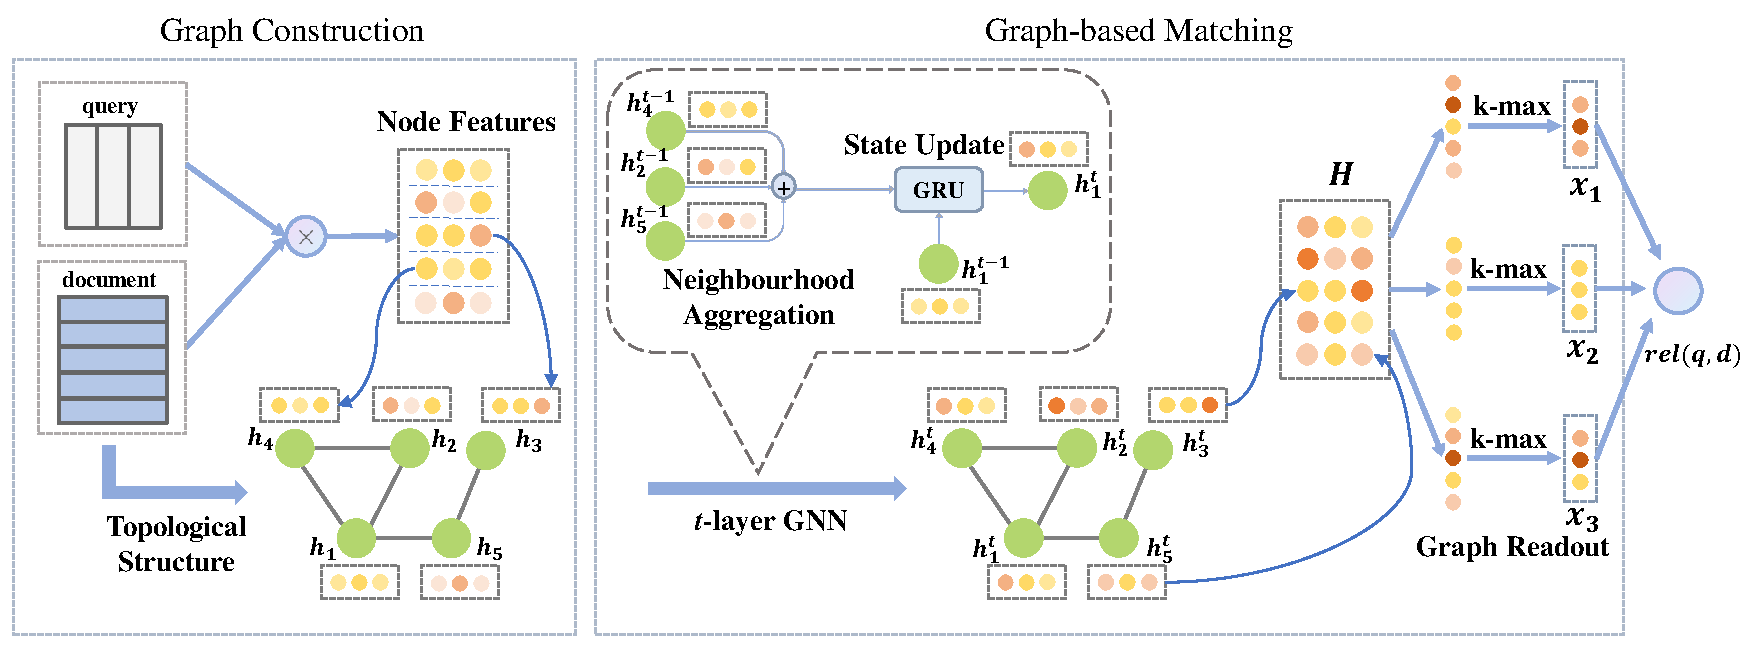
\includegraphics[width=\textwidth]{./pics/grmm.pdf}
	\caption{The workflow of the GRMM model. The document is first transformed into the graph-of-word form, where the node feature is the similarity between the word and each query term. Then, graph neural networks are applied to propagate these matching signals on the document graph. Finally, to estimate a relevance score, top-$k$ signals of each query term are chosen to filter out irrelevant noisy information, and their features are fed into a dense neural layer. }
	\label{fig:2} 
\end{figure*}

Nevertheless, the majority of existing neural matching models only take the linear text sequence, inevitably limiting the model capability. To this end, we propose to break the linear text format and represent the document in a flexible graph structure, where comprehensive interactions can be explicitly modeled. 



\subsection{Graph Neural Networks}
Graph is a kind of data structure which cooperates with a set of objects (nodes) and their relationships (edges). Recently, researches of analysing graphs with machine learning have attracted much attention because of its great representative power in many fields. 

Graph neural networks (GNNs) are deep learning based methods that operate in the graph domain. The concept of GNNs is previously proposed by  \cite{scarselli2008graph}. Generally, nodes in GNNs update own hidden states by aggregating neighbourhood information and mixing things up into a new context-aware state. There are also many variants of GNNs with various kinds of aggregators and updaters, such as \cite{li2016gated,kipf2017semi,hamilton2017inductive,velivckovic2018graph}. 

Due to the convincing performance and high interpretability, GNNs have become a widely applied structural analysis tool. Recently, there are many applications covering from recommendation \cite{wu2019session,li2019fi} to NLP area, including text classification \cite{yao2019graph,zhang2020every}, question answering \cite{de2019question}, and spam review detection \cite{li2019spam}.

In this work, we employ GNNs in the relevance matching task to extract implicit matching patterns from the query-document interaction signals, which is intrinsically difficult to be revealed by existing methods. 



\section{Proposed Method}

In this section, we introduce thoroughly our proposed Graph-based Relevance Matching Model (GRMM). We first formulate the problem and demonstrate how to construct the graph-of-word formation from the query and document, and then describe the graph-based matching method in details. Figure \ref{fig:2} illustrates the overall process of our proposed architecture.

\subsection{Problem Statement}
Given a query $q$ and a document $d$, they are represented as a sequence of  words 
$q=\left[w_{1}^{(q)}, \ldots, w_{M}^{(q)}\right]$  and $d=\left[w_{1}^{(d)}, \ldots, w_{N}^{(d)}\right]$, where $w_{i}^{(q)}$ denotes the $i$-th word in the query, $w_{i}^{(d)}$ denotes the $i$-th word in the document, $M$ and $N$ denote the length of the query and the document respectively.
The aim is to compute a relevance score $rel(q,d)$ regarding the query words and the document words.


\subsection{Graph Construction}
\label{sec:graphconstruct}
To leverage the long-distance term dependency information, the first step is to construct a graph $\mathcal{G}$ for the document. It typically consists of two components denoted as $\mathcal{G}=(\mathcal{V}, \mathcal{E})$, 
where $\mathcal{V}$ is the set of vertexes with \emph{node features}, and $\mathcal{E}$ is the set of edges as the \emph{topological structure}.

\subsubsection{Node features.}
We represent each unique word instead of sentence or paragraph in the document as a node. Thus the word sequence is squeezed to a node set $\left\{w_{1}^{(d)}, \ldots, w_{n}^{(d)}\right\}$, where $n$ is the number of unique words in the document ($|\mathcal{V}| = n  \leq N$). Each node feature is set the interaction signal between its word embedding and query term embeddings. We simply employ the cosine similarity matrix as the interaction matrix, denoted as $\mathbf{S} \in \mathbb{R}^{n \times M}$, where each element $\mathbf{S}_{ij}$ between document node $w^{(d)}_i$ and query term $w^{(q)}_j$ is defined as:
\begin{equation}\mathbf{S}_{i j}=cosine\left(\mathbf{e}_i^{(d)}, \mathbf{e}_j^{(q)}\right)
\end{equation}
where $\mathbf{e}_{i}^{(d)}$ and $\mathbf{e}_{j}^{(q)} $ are embedding vectors for $w_{i}^{(d)}$ and $w_{j}^{(q)}$ respectively. In this work, we use word2vec \cite{mikolov2013distributed} technique to convert words into dense and semantic embedding vectors.

\subsubsection{Topological structure.}
In addition to the node feature matrix, the adjacency matrix representing the topological structure constitutes for the graph as well. The structure generally describes the connection between the nodes and reveals their relationships. We build bi-directional connections for each pair of word nodes that co-occur within a sliding window, along with the original document word sequence $d$. By restricting the size of the window, every word can connect with their neighbourhood words which may share related contextual meanings. However, GRMM differs from those local relevance matching methods in that the combined word node can bridge all neighbourhoods together and therefore possess a document-level receptive field. In other words, it breaks the constraints of local context and can model the long-distance word dependencies that we concern. Note that in the worst case where there are no duplicate words, the graph would still perform as a sequential and local scheme. 

Formally, the adjacency matrix $\mathbf{A} \in \mathbb{R}^{n \times n}$ is defined as:
\begin{equation}
\mathbf{A}_{i j}=\left\{\begin{array}{ll}
count(i, j) & \text{if } i \not= j \\
0 & \text{otherwise}
\end{array}\right.
\end{equation}
where $count(i, j)$ is the number of times that the words $w_{i}^{(d)}$ and $w_{j}^{(d)}$ appear in the same sliding window. To alleviate the exploding/vanishing gradient problem \cite{kipf2017semi}, we normalise the adjacency matrix as $\tilde{\mathbf{A}} = \mathbf{D}^{-\frac{1}{2}} \mathbf{A} \mathbf{D}^{-\frac{1}{2}}$, where $\mathbf{D} \in \mathbb{R}^{n \times n}$ is the diagonal degree matrix and $\mathbf{D}_{ii} = \sum_j \mathbf{A}_{ij}$.



\subsection{Graph-based Matching}
Once we obtain the graph $\mathcal{G}$, we focus on making use of its node features and structure information with graph neural networks. In particular, the query-document interaction and the intra-document word interaction are learned mutually following the procedures - \emph{neighbourhood aggregation}, \emph{state update} and \emph{feature election}. 

\subsubsection{Neighbourhood Aggregation.}
As discussed in Section \ref{sec:graphconstruct}, we initialise the node state $\mathbf{h}^0_i$ with the query-document interaction matrix:
\begin{equation}\mathbf{h}^0_i =  \mathbf{S}_{i,:}
\end{equation}
where $\forall i\in [1, n]$ denotes the $i$-th node in the graph, and $\mathbf{S}_{i,:}$ is the $i$-th row of the interaction matrix $\mathbf{S}$.

Assume each word node either holds the core information or serves as a bridge connecting others, it is necessary to make the information flow and enrich the related fractions on the graph.
Through propagating the state representations to a node from its neighbours, it can receive the contextual information within the first-order connectivity as:
\begin{equation}\mathbf{a}_{i}^{t}=\sum_{(w_{i}, w_{j}) \in \mathcal{E}} \mathbf{\tilde{A}}_{ij} \mathbf{W}_{a} \mathbf{h}_{j}^{t}\end{equation}
where $\mathbf{a}_i^t \in \mathbb{R}^{M}$ denotes the summed message from neighbours, $t$ denotes the current timestamp, and $\mathbf{W}_a$ is a trainable transformation matrix to project features into a new relation space. When aggregate $t$ times recursively, a node can receive the information propagated from its $t$-hop neighbours. In this way, the model can achieve \emph{high-order aggregation} of the query-document interaction as well as the intra-document interaction.

\subsubsection{State Update.}
To incorporate the contextual information into the word nodes, we engage a GRU-like function \cite{li2016gated} to automatically adjust the merge proportion of its current representation $\mathbf{h}^{t}_i$ and the received representation $\mathbf{a}^{t}_i$, which is formulated as:
\begin{equation}\begin{array}{l}
\mathbf{z}_{i}^{t}=\sigma\left(\mathbf{W}_{z} \mathbf{a}_{i}^{t}+\mathbf{U}_{z} \mathbf{h}_{i}^{t}+\mathbf{b}_{z}\right)
\end{array}\end{equation}
\begin{equation}
\mathbf{r}_{i}^{t}=\sigma\left(\mathbf{W}_{r} \mathbf{a}_{i}^{t}+\mathbf{U}_{r} \mathbf{h}_{i}^{t}+\mathbf{b}_{r}\right)
\end{equation}
\begin{equation}\tilde{\mathbf{h}}_{i}^{t}=\tanh \left(\mathbf{W}_{h} \mathbf{a}_{i}^{t}+\mathbf{U}_{h}\left(\mathbf{r}_{i}^{t} \odot \mathbf{h}_{i}^{t}\right)+\mathbf{b}_{h}\right)\end{equation}
\begin{equation}\mathbf{h}_{i}^{t+1}=\tilde{\mathbf{h}}_{i}^{t} \odot \mathbf{z}_{i}^{t}+\mathbf{h}_{i}^{t} \odot\left(1-\mathbf{z}_{i}^{t}\right)\end{equation}
where $\sigma(\cdot)$ is the sigmoid function, $\odot$ is the Hardamard product operation, tanh$(\cdot)$ is the non-linear tangent hyperbolic activation function, and all $\mathbf{W_*, U_*}$ and $\mathbf{b_*}$ are trainable weights and biases. 

Specifically, $\mathbf{r}^{t}_i$ determines irrelevant information for hidden state $\tilde{\mathbf{h}}^{t}_i$ to forget (reset gate), while $\mathbf{z}^{t}_i$ determines which part of past information to discard and which to push forward (update gate). With the layer $t$ going deep, high-order information becomes complicated, and it is necessary to identify useful dependencies with the two gates. We have also tried plain updater such as GCN \cite{kipf2017semi} in our experiments but did not observe satisfying performance due to its simplicity.


\subsubsection{Graph Readout.}
The last phase involves locating the position where relevance matching happens as a delegate for the entire graph. Since it is suggested that not all words make contributions, and some may cause adverse influences \cite{guo2016deep}, here we only select the most informative features to represent the query-document matching signals. Intuitively, higher similarity means higher relevance possibility. Hence we perform a $k$-max-pooling strategy over the query dimension and select the top $k$ signals for each query term, which also prevents the model from being biased by the document length. The formulas are expressed as:
\begin{equation}\mathbf{H}=\mathbf{h}_{1}^{t} \parallel \mathbf{h}_{2}^{t} \parallel \ldots \parallel \mathbf{h}_{n}^{t}\end{equation}
\begin{equation}
\mathbf{x}_{j} = {topk}(\mathbf{H}_{:,j})
\end{equation}
where $\forall j\in [1, M]$ denotes the $j$-th query term, and $\mathbf{H}_{:,j}$ is the $j$-th column of the feature matrix $\mathbf{H}$.

\subsection{Matching Score and Training}
After obtaining low-dimensional and informative matching features $\mathbf{x}_j$, we move towards converting them into actual relevance scores for training and inference. Considering different terms may have different importances \cite{guo2016deep}, we assign each with a soft gating network as:
\begin{equation}g_{j}=\frac{\exp \left({c} \cdot idf_j \right)}{\sum_{j=1}^{M} \exp \left({c} \cdot idf_j \right)}\end{equation}
where $g_j$ denotes the term weight, $idf_j$ is the inverse document frequency of the $j$-th query term, and $c$ is a trainable parameter. To reduce the amount of parameters and avoid over-fitting, we score each query term with a weight-shared multi-layer perceptron (MLP) and sum them up as the final result:
\begin{equation}{rel}(q, d)=\sum_{j=1}^{M} g_j \cdot \tanh \left(\mathbf{W}_x \mathbf{x}_{j}+{b}_x \right)\end{equation}
where $\mathbf{W}_x, b_x$ are trainable parameters for MLP.

Finally, we adopt the pairwise hinge loss which is commonly used in information retrieval to optimise the model parameters:
\begin{small}
	\begin{equation}\mathcal{L}\left(q, d^{+}, d^{-}\right)=\max \left(0, 1-rel\left(q, d^{+}\right)+rel\left(q, d^{-}\right)\right)\end{equation} 
\end{small}
where $\mathcal{L}\left(q, d^{+}, d^{-}\right)$ denotes the pairwise loss based on a triplet of the query $q$, a relevant (positive) document sample $d^+$, and an irrelevant (negative) document sample $d^-$.



\section{Experiments}



We compare 11 representative machine learning models, including GNN and GNN-RNN, on US county-level crop yields for corn and soybean. We evaluate performance on three metrics: RMSE, $R^2$, and correlation coefficient. Given a test year $t$, we use year $t-1$ for validation and all the prior years for training. For example, if the test year is 2019, we train on data from years 1981-2017 (inclusive), validate on 2018 crop yields, and test on 2019 crop yields.

\subsection{Dataset Details}

% NOte: see dataset_OLD.tex for more detailed text, if we need it in the future

Crop yield labels for corn and soybean are available from the USDA Crop Production Reports \cite{usda2013national} for numerous counties in the US. Not all counties report data in every year, but the coverage is still quite comprehensive. For example, for corn, all years between 1981 and 2003 have over 2,000 counties across $41$ states reporting data. We train and evaluate our model on all counties where yield data is available. (When computing the loss, we ignore counties that do not have yield labels for that year.)

We use a variety of climate, land surface, and soil quality variables as input features; these features are available for almost all counties in the contiguous 48 US states (3,107 counties in total\footnote{The only exception is Nantucket County, Massachusetts, where land surface model data is missing, since it is an offshore island. Also note that some counties have feature data but not label (yield) data. Only the GNN and GNN-RNN models can make use of these unlabeled county features.}). We draw 7 weather features from the PRISM climate mapping system \cite{daly2013prism}: precipitation, min/mean/max temperature, min/max vapor pressure deficit, and mean dewpoint temperature. These features are available at a $4 \times 4$ km grid for each day. 

We acquire 16 land surface features from the North American Land Data Assimilation System (NLDAS) \cite{xia2012continental}, which is a large-scale land surface model that closely simulates land surface parameters. These features include soil moisture content, moisture availability, and soil temperature (all at various soil depths), as well as observed weather variables such as wind speed and humidity. These variables are available at a $0.125 \times 0.125$ degree ($\sim 14$ km) spatial resolution, every hour. 

%We aggregate the hourly data to daily, and aggregate the grid to the county level in the same way as PRISM. 


% We acqui  gSSURGO dataset \cite{soil2019gridded} provides abundant survey-collected features regarding the soil composition and quality of an area. These gridded features are available at a 30-meter spatial resolution, and \emph{do not change over time}.

Soil quality features were acquired from the Gridded Soil Survey Geographic Database (gSSURGO) \cite{soil2019gridded}, at a $30 \times 30$ meter resolution. These features include available water capacity, bulk density, and electrical conductivity, pH, and organic matter.
% We used 20 features that are available at 6 different soil depth levels, as well as 6 ``extra'' features (such as crop productivity indices) that are not depth-dependent. 
Unlike the weather and land surface features, the gSSURGO soil quality features are fixed and \emph{do not change over time}. In addition to the raw features, we use the raw sand, silt, and clay percentages to compute the ``soil texture type'' of each pixel based on the Natural Resources Conservation Service Soil Survey's classification scheme \cite{soiltexture}, and then compute the fraction of each county occupied by each soil texture type. In total, we have a total of 20 gSSURGO variables that are depth-dependent (so there are values for 6 different soil depth levels), and 6 ``extra'' variables which are not depth-dependent (such as crop productivity indices). Finally, as in \cite{khaki2020cnn}, we use the average crop yield (over all counties) of the previous year as an additional input feature, to capture the increasing trend in crop yield over time. A full list of the features can be found in the Appendix.

%Again, we aggregate these features to the county level using the weighted-average technique, only considering pixels that are cropland/grassland/pasture.
% The North American Land Data Assimilation System (NLDAS) \cite{xia2012continental} is a large-scale land surface model that closely simulates land surface parameters. We collect 16 features from this dataset, including several ``forcing'' weather variables, as well as soil moisture, moisture availability, and soil temperature at multiple soil depths. These data are originally available at a $0.125 \times 0.125$ degree (roughly $14$ km) spatial resolution, and an hourly temporal resolution. We aggregate the hourly data to daily, and aggregate the grid to the county level in the same way as PRISM. 


All of these datasets were originally available as gridded raster data at a variety of spatial resolutions. We aggregated each feature to the county level by computing the weighted average of the variable over all grid cells that overlap with the county. Each grid cell is weighted by the percentage of the cell that lies inside the county, multiplied by the percentage of that grid cell which is cropland, pasture, or grassland; the land cover percentages are computed using the National Land Cover Database \cite{nlcd}. In addition, the time-dependent variables (weather and land surface) were aggregated from daily to weekly frequency to make the prediction task more tractable.

%Figure \ref{aggregating_to_county} shows an example of the process we use to aggregate gridded features to the county level.

% \begin{figure}[t]
% \centering
% \includegraphics[width=0.75\columnwidth]{figs/nldas.png}
% \includegraphics[width=0.75\columnwidth]{figs/nldas_SOILM_layer1_19810101_county.png}
% \caption{Example of aggregating features to county level. \\
% \textbf{(a)} raw raster of soil moisture from NLDAS. \\
% \textbf{(b)} Percentage cropland/grassland/pasture (used to compute grid cell weights).\\
% \textbf{(c)} the county-level values we generated. \textbf{make bigger, make size of figures consistent}}
% \label{aggregating_to_county}
% \end{figure}

\subsection{Compared Methods}

We consider two types of methods: \textbf{(a) single-year methods} that only use features from year $t$ to predict yield for the same year $t$, and \textbf{(b) 5-year methods} that use features from a 5-year series (years $\{t-4, t-3, \dots, t\}$) to predict yield for year $t$.

\textbf{Single-year methods.} We first consider methods that only use a single year of data to make predictions, to provide a fair comparison to the single-year GNN. For non-deep baseline methods, we select lasso, ridge regressor and gradient boosting regressor. For these methods, we flatten all the features from the entire year into a single feature vector, ignoring the temporal and soil-depth structure in the data.
Next, we tried three baseline deep learning architectures for $f_{wl}(\cdot)$: LSTM \cite{hochreiter1997long}, GRU \cite{chung2014empirical}, and 1-D CNN \cite{kalchbrenner2014convolutional}. All of these methods process the weekly time-series of weather and land surface data within the year. We compare these methods with our single-year GNN model (Eq. \ref{eq:gnn}), which incorporates geospatial context in making predictions.
 
\textbf{5-year methods.} For history-dependent models, we follow \cite{khaki2020cnn} by considering a 5-year dependency for a consistent and fair comparison. Two baseline models using LSTM and GRU respectively handle the raw inputs $\{\mathbf{x}_{c,t-\Delta t}, ...,\mathbf{x}_{c,t}\}$ directly with $r(\cdot)$. Specifically, they flatten the features \emph{for each year} into a single vector (disregarding the weekly structure of the weather data or the depth structure of the soil data), and then feed the 5 year-vectors into the LSTM or GRU. The most recent CNN-RNN model \cite{khaki2020cnn} pre-processes the raw features with a CNN (choosing CNN for $f_{wl}(\cdot)$) and then uses a LSTM to model the sequence embeddings as described in Eq. \ref{eq:rnn}. Finally, the GNN-RNN model proposed in this paper (Eq. \ref{eq:gnn-rnn}) still uses a CNN for $f_{wl}(\cdot)$ to encode the raw features into an embedding for each year, then uses the GNN to refine the embeddings using information from the county's spatial context, and then passes those embeddings into an LSTM.

% Two additional methods proposed in this paper are single year GNN (Eq. \ref{eq:gnn}) and GNN-RNN (Eq. \ref{eq:gnn-rnn}).


\subsection{Evaluation Metrics}
We evaluate all methods on three popular metrics for regression: root mean square error (RMSE), the coefficient of determination ($R^2$), Pearson correlation coefficient (Corr). RMSE and $R^2$ tell us how well a regression model can predict the value of the response variable in absolute terms and percentage terms respectively. Note that our RMSE figures are expressed in units of the standard deviation of that crop's yield (across all years). Corr is essentially a normalized measurement of the covariance between two sets of data, and captures the strength of the linear correlation between true and predicted values. See Appendix for formal definitions.


\begin{table*}[tb]
\centering
\subfloat[2018 corn results]{
\begin{tabular}{|l|c|c|c|} \hline
\textbf{Method} & \textbf{RMSE} & \textbf{$R^2$} & \textbf{Corr} \\ \hline
% \multicolumn{4}{|l|}{\textbf{1-year methods}} \\ \hline
lasso 1y & 0.7846 & 0.3839 & 0.7778 \\
ridge 1y & 0.9255 & 0.1428 & 0.7626 \\
gradient-boosting 1y & 0.7402 & 0.4516 & 0.7794 \\
gru 1y & 0.5938 & 0.6472 & 0.8158 \\
lstm 1y & 0.6146 & 0.6220 & 0.8303 \\
cnn 1y & 0.5824 & 0.6606 & 0.8235 \\ \hdashline
gnn 1y \textbf{(ours)} & \textbf{0.4846} & \textbf{0.7517} & \textbf{0.8759} \\
\fontsize{9}{10}\selectfont
\std{std} & \std{0.0097} & \std{0.0100} & \std{0.0019}
\fontsize{10}{10}\selectfont\\
\hline %\Xhline{1.5pt} 
% \multicolumn{4}{|l|}{\textbf{5-year methods}} \\ \hline
gru 5y & 0.6765 & 0.5419 & 0.8194 \\
lstm 5y & 0.6542 & 0.5716 & 0.8060 \\
cnn-rnn 5y & 0.5511 & 0.6936 & 0.8425 \\ \hdashline
gnn-rnn 5y \textbf{(ours)} & \textbf{0.4900} & \textbf{0.7595}  & \textbf{0.8731} \\ 
\fontsize{9}{10}\selectfont
\std{std} & \std{0.0191} & \std{0.0186} & \std{0.0092} 
\fontsize{10}{10}\selectfont \\ \hline
\end{tabular}
} \qquad
\subfloat[2019 corn results]{
\begin{tabular}{|l|c|c|c|} \hline
\textbf{Method} & \textbf{RMSE} & \textbf{$R^2$} & \textbf{Corr} \\ \hline
lasso 1y & 0.6838 & 0.3122 & 0.6715 \\
ridge 1y & 0.7081 & 0.2623 & 0.6723 \\
gradient-boosting 1y & 0.7345 & 0.2064 & 0.6857 \\
gru 1y & 0.5890 & 0.4897 & 0.7381 \\
lstm 1y & 0.6245 & 0.4262 & 0.7096 \\
cnn 1y & 0.5572 & 0.5432 & 0.7384 \\ \hdashline
gnn 1y \textbf{(ours)} & \textbf{0.4930} & \textbf{0.6286} & \textbf{0.8011} \\
\fontsize{9}{10}\selectfont
\std{std} & \std{0.0068} & \std{0.0102} & \std{0.0037}
\fontsize{10}{10}\selectfont\\ \hline
gru 5y & 0.5279 & 0.5900 & 0.7785 \\
lstm 5y & 0.5311 & 0.5849 & 0.7821 \\
cnn-rnn 5y & 0.5212 & 0.5842 & 0.7868 \\ \hdashline
gnn-rnn 5y \textbf{(ours)} & \textbf{0.4677} & \textbf{0.6782} & \textbf{0.8272} \\
\std{std} & \std{0.0035} & \std{0.0049} & \std{0.0038} \\ \hline
\end{tabular}
} \\
\subfloat[2018 soybean results]{
\begin{tabular}{|l|c|c|c|} \hline
\textbf{Method} & \textbf{RMSE} & \textbf{$R^2$} & \textbf{Corr} \\ \hline
lasso 1y & 0.6226 & 0.6090 & 0.7912 \\
ridge 1y & 0.7633 & 0.4125 & 0.7550 \\
gradient-boosting 1y & 0.6686 & 0.5492 & 0.7986 \\
gru 1y & 0.6376 & 0.5932 & \textbf{0.8356} \\
lstm 1y & 0.6459 & 0.5825 & 0.8129 \\
cnn 1y & 0.6584 & 0.5661 & 0.7988 \\ \hdashline
gnn 1y \textbf{(ours)} & \textbf{0.5637} & \textbf{0.6794} & 0.8273 \\
\fontsize{9}{10}\selectfont
\std{std} & \std{0.0144} & \std{0.0163} & \std{0.0095}
\fontsize{10}{10}\selectfont\\ \hline
 % \Xhline{1.5pt}
gru 5y & 0.6094 & 0.6254 & 0.8218 \\
lstm 5y & 0.5430 & 0.7026 & 0.8459 \\
cnn-rnn 5y & 0.5647 & 0.6784 & \textbf{0.8650} \\ \hdashline
gnn-rnn 5y \textbf{(ours)} & \textbf{0.5333} & \textbf{0.7129} & 0.8591 \\ 
\fontsize{9}{10}\selectfont
\std{std} & \std{0.0194} & \std{0.0206} & \std{0.0049} 
\fontsize{10}{10}\selectfont
\\ \hline

\end{tabular}
} \qquad
\subfloat[2019 soybean results]{
\begin{tabular}{|l|c|c|c|} \hline
\textbf{Method} & \textbf{RMSE} & \textbf{$R^2$} & \textbf{Corr} \\ \hline
lasso 1y & 0.5731 & 0.6137 & 0.8089 \\
ridge 1y & 0.6069 & 0.5668 & 0.7944 \\
gradient-boosting 1y & 0.6802 & 0.4558 & 0.7899 \\
gru 1y & 0.5742 & 0.5150 & 0.7569 \\
lstm 1y & 0.5907 & 0.4867 & 0.7195 \\
cnn 1y & 0.5699 & 0.5222 & 0.7385 \\ \hdashline
gnn 1y \textbf{(ours)} & \textbf{0.4916} & \textbf{0.7148} & \textbf{0.8505} \\
\fontsize{9}{10}\selectfont
\std{std} & \std{0.0335} & \std{0.0395} & \std{0.0165}
\fontsize{10}{10}\selectfont \\ \hline
gru 5y & 0.5751 & 0.6109 & 0.8158 \\
lstm 5y & 0.5512 & 0.6427 & 0.8156 \\
cnn-rnn 5y & 0.5365 & 0.6615 & 0.8423 \\ \hdashline
gnn-rnn 5y \textbf{(ours)}  & \textbf{0.4745} & \textbf{0.7349} & \textbf{0.8602} \\
% lasso 1y & 0.6838 & 0.3122 & 0.6715 \\
% ridge 1y & 0.7081 & 0.2623 & 0.6723 \\
% gradient-boosting 1y & 0.7345 & 0.2064 & 0.6857 \\
% gru 1y & 0.5890 & 0.4897 & 0.7381 \\
% lstm 1y & 0.6245 & 0.4262 & 0.7096 \\
% cnn 1y & 0.5572 & 0.5432 & 0.7384 \\
% gnn 1y & \textbf{0.4930} & \textbf{0.6286} & \textbf{0.8011} \\ \Xhline{1.5pt} 
% gru 5y & 0.5751 & 0.6109 & 0.8158 \\
% lstm 5y & 0.5512 & 0.6427 & 0.8156 \\
% cnn-rnn 5y & 0.5212 & 0.5842 & 0.7868 \\ \hline
% gnn-rnn 5y & \textbf{0.4679} & \textbf{0.6777} & \textbf{0.8274} \\
\fontsize{9}{10}\selectfont
\std{std} & \std{0.0160} & \std{0.0179} & \std{0.0076}
\fontsize{10}{10}\selectfont \\ \hline
\end{tabular}
}
\caption{Evaluation results. For RMSE, lower is better; for $R^2$ and Corr, higher is better. We grouped the methods based on whether they use 1 year of data (1y) or 5 years of data (5y) to make predictions.}
\label{results}
\end{table*}



\subsection{Model Details}

For the shallow models (ridge regression, lasso, and gradient boosting regressor), we used scikit-learn's implementations. 

For the baseline single-year models, we evaluated using LSTM, GRU, and CNN as $f_{wl}(\cdot)$ to process the weekly weather and land surface data. For CNN, we used a 1-D CNN similar to the one in \cite{khaki2020cnn}, but we process all weather and land surface parameters together. The CNN contains series of 1D convolutions, ReLUs, and average pooling layers; this sequence is repeated four times.  For all methods that use LSTM or GRU, we used PyTorch's implementation with 64 hidden states.


The same CNN is used as the encoder for the weekly weather and land surface data in the CNN-RNN, GNN, and GNN-RNN models. (We also tried using an LSTM as the encoder for the weekly data for these models, but  this did not improve results.) For all methods except for the 5-year LSTM/GRU, we processed the soil data using another small 1-D CNN (with three convolutional layers, and without average pooling), where the convolutions operate across 6 different soil depths.

%For the CNN-RNN model, the CNNs described earlier are used to encode each year's features into an embedding. Then the embeddings for the five years are passed through an LSTM.

For the simple 5-year baseline models (LSTM and GRU), we fed the flattened feature vectors for each year through an LSTM or GRU, followed by a 2-layer fully connected network.


For the GNN and GNN-RNN models, we used the implementation of GraphSAGE from the dgl library; we used a 2-layer GNN, with edge dropout of 0.1. The adjacency graph of US counties is provided by the US Census Bureau. We used stochastic mini-batch training to train the model, where each layer samples 10 neighbors to receive messages from. We tried different aggregation functions and found that the ``pooling'' approach generally performed best.

%The GNN-RNN model considers a sequence of 5 years; the GNN is applied on every year to refine the embeddings produced by the CNN encoder with information from neighboring counties. Then the embeddings outputted by the GNN are fed into a final LSTM and then a fully-connected layer.

For all methods, we use the Adam optimizer \cite{kingma2014adam}, sometimes with a mild cosine or step decay. We tried learning rates between 1e-5 and 1e-3, used a weight decay of 1e-5 or 1e-4, and a batch size of 32, 64, or 128. We trained the model  for 100 to 200 epochs (until the validation loss clearly stopped improving). We chose the epoch and hyperparameter setting that produced the lowest RMSE on the validation year (the year before the test year).  We ran the GNN and GNN-RNN models 3 times with different random seeds to evaluate the variance in the results. The Appendix contains more details about hyperparameters. 


%\junwen{Just for GNN-RNN (required by submission checklist): (1) The number of algorithm runs used to compute each reported result. (2) Analysis of experiments goes beyond single-dimensional summaries of performance.(std) (3) lists all final (hyper-)parameters used for each model. \\ We could put some of these to Appx.}


% \begin{table}[]
% \centering
% % \fontsize{9}{10}\selectfont
% \begin{tabular}{|l|c|c|c|} \hline
% \textbf{Method} & \textbf{RMSE} & \textbf{$R^2$} & \textbf{Corr} \\ \hline
% gru 1y & 0.5890 & 0.4897 & 0.7381 \\
% lstm 1y & 0.6245 & 0.4262 & 0.7096 \\
% cnn 1y & 0.5572 & 0.5432 & 0.7384 \\
% gnn 1y & \textbf{0.4930} & \textbf{0.6286} & \textbf{0.8011} \\ \hline
% lasso 5y & 0.6838 & 0.3122 & 0.6715 \\
% ridge 5y & 0.7081 & 0.2623 & 0.6723 \\
% gradient-boosting 5y & 0.7345 & 0.2064 & 0.6857 \\
% gru 5y & 0.5751 & 0.6109 & 0.8158 \\
% lstm 5y & 0.5512 & 0.6427 & 0.8156 \\
% cnn-rnn 5y & 0.5212 & 0.5842 & 0.7868 \\
% gnn-rnn 5y & \textbf{0.4679} & \textbf{0.6777} & \textbf{0.8274} \\ \hline
% \end{tabular}
% \caption{2019 corn results}
% \label{2019_corn}
% \end{table}

% \begin{table}[]
% \centering
% \fontsize{9}{10}\selectfont
% \begin{tabular}{|l|c|c|c|} \hline
% \textbf{Method} & \textbf{RMSE} & \textbf{$R^2$} & \textbf{Corr} \\ \hline
% gru 1y & 0.6376 & 0.5932 & 0.8356 \\
% lstm 1y & 0.6459 & 0.5825 & 0.8129 \\
% cnn 1y & 0.6584 & 0.5661 & 0.7988 \\
% gnn 1y & \textbf{0.5852} & \textbf{0.6547} & \textbf{0.8175} \\ \hline
% lasso 5y & 0.6226 & 0.6090 & 0.7912 \\
% ridge 5y & 0.7633 & 0.4125 & 0.7550 \\
% gradient-boosting 5y & 0.6686 & 0.5492 & 0.7986 \\
% gru 5y & 0.6094 & 0.6254 & 0.8218 \\
% lstm 5y & 0.5430 & 0.7026 & 0.8459 \\
% cnn-rnn 5y & 0.5647 & 0.6784 & \textbf{0.8650} \\
% gnn-rnn 5y & \textbf{0.5333} & \textbf{0.7129} & 0.8591 \\ \hline
% \end{tabular}
% \caption{2018 soybean results}
% \label{2018_soybean}
% \end{table}

% \begin{table}[]
% \centering
% \fontsize{9}{10}\selectfont
% \begin{tabular}{|l|c|c|c|} \hline
% \textbf{Method} & \textbf{RMSE} & \textbf{$R^2$} & \textbf{Corr} \\ \hline
% gru 1y & 0.5742 & 0.5150 & 0.7569 \\
% lstm 1y & 0.5907 & 0.4867 & 0.7195 \\
% cnn 1y & 0.5699 & 0.5222 & 0.7385 \\
% gnn 1y & \textbf{0.5170} & \textbf{0.6856} & \textbf{0.8299} \\ \hline
% lasso 5y & 0.5731 & 0.6137 & 0.8089 \\
% ridge 5y & 0.6069 & 0.5668 & 0.7944 \\
% gradient-boosting 5y & 0.6802 & 0.4558 & 0.7899 \\
% gru 5y & 0.5751 & 0.6109 & 0.8158 \\
% lstm 5y & 0.5512 & 0.6427 & 0.8156 \\
% cnn-rnn 5y & 0.5365 & 0.6615 & 0.8423 \\
% gnn-rnn 5y & \textbf{0.5091} & \textbf{0.6951} & \textbf{0.8434} \\ \hline
% \end{tabular}
% \caption{2019 soybean results}
% \label{2019_soybean}
% \end{table}



\begin{table}[t]
\centering
\begin{tabular}{|l|c|c|c|} \hline
\textbf{Method} & \textbf{RMSE} & \textbf{$R^2$} & \textbf{Corr} \\ \hline
lstm 1y & 0.6347 & 0.5968 & \textbf{0.8148} \\
cnn 1y & 0.7253	& 0.4736 & 0.7004 \\
gnn 1y \textbf{(ours)} & \textbf{0.5877} & \textbf{0.6543} & 0.8124 \\ \hline
lstm 5y & 0.7004 & 0.5091 & 0.7708 \\
cnn-rnn 5y & 0.6532 & 0.5730 & 0.7732 \\
gnn-rnn 5y \textbf{(ours)} & \textbf{0.5836} & \textbf{0.6591} & \textbf{0.8259} \\ \hline
\end{tabular}
\caption{Early prediction results (2018 corn, after June 1).}
\label{early}
\end{table}

\subsection{Crop Yield Prediction Results}
% Can use https://www.tablesgenerator.com/latex_tables to generate tables from Google sheets


\begin{figure}[bt]
\centering
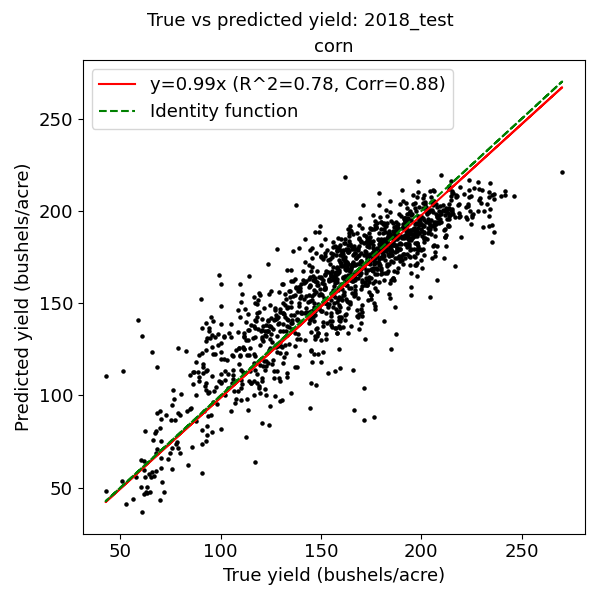
\includegraphics[width=0.8\columnwidth]{figs/true_vs_predicted_scatter_corn_2018_test.png}
\caption{Predicted vs. ground truth corn yields in 2018}
\label{scatter}
\end{figure}

\begin{figure}[tb]
\centering
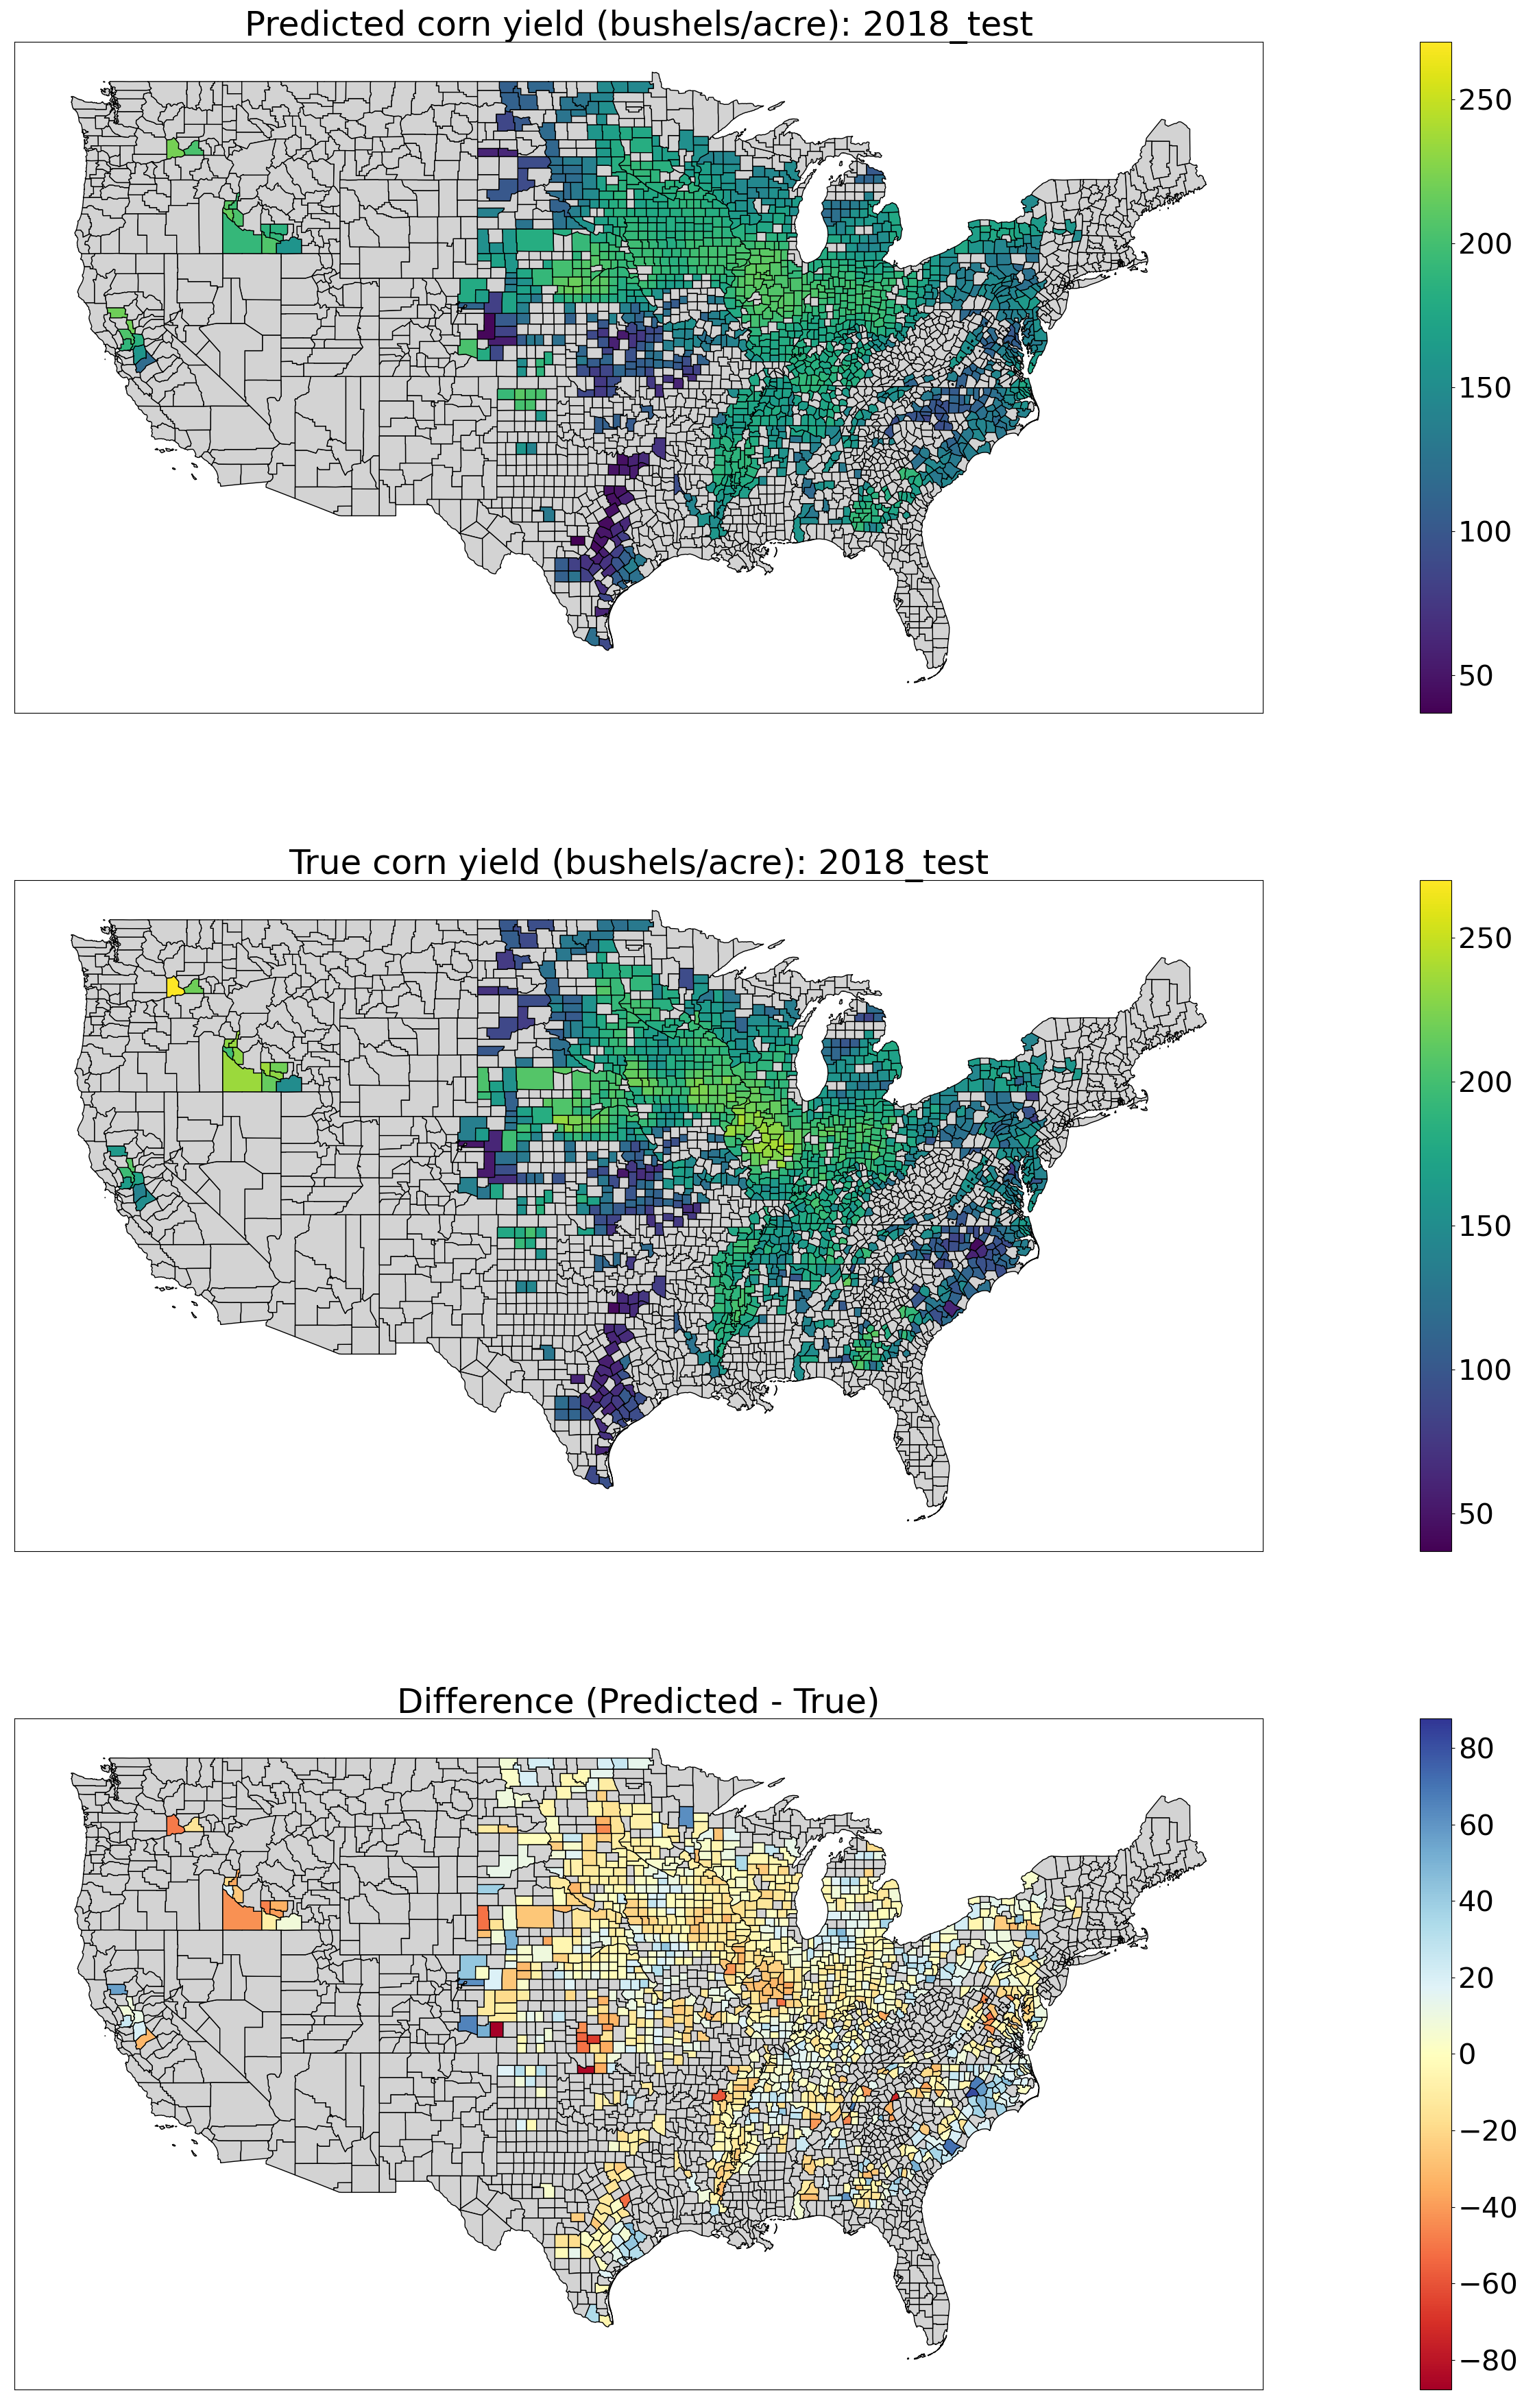
\includegraphics[width=0.95\columnwidth]{figs/true_vs_predicted_map_corn_2018_test.png}
\caption{Maps of predicted (top) and true (middle) corn yields in 2018, along with the difference (bottom). For the Difference plot, yellow means an accurate prediction, blue means the model predicted too high, and red means the model predicted too low. Gray means no data.}
\label{map}
\end{figure}

We evaluate the model on four test datasets: 2018 corn, 2018 soybean, 2019 corn, and 2019 soybean. These datasets span a wide geographic area, as well as differing growing conditions (2019 was a bad year due to the wet spring in the Midwest, which caused planting to be delayed). The results on these datasets are shown in Table \ref{results}. For the methods that only use 1 year when making predictions, our GNN model clearly outperforms comparable baselines across all datasets and metrics (except for 2018 soybean Corr, where it is slightly worse than GRU). For the methods that use a history of 5 years, our GNN-RNN outperforms competing baselines in almost all cases (except for 2018 soybean Corr, where it is slightly worse than CNN-RNN). For example, in 2019, our corn yield prediction on $R^2$ score is 16\% better than the prediction of a state-of-the-art work \cite{khaki2020cnn}. On average, we achieve a relative $R^2$ improvement of 10.44\% over the recent CNN-RNN model, 16.16\% over the 5-year LSTM, and a relative RMSE improvement of 9.6\% over the CNN-RNN model, 13.18\% over the 5-year LSTM.  These indicate the importance of exploiting geospatial context in making these predictions.




Figure \ref{scatter} shows an example scatterplot of true vs. predicted corn yields for the test year 2018. The GNN-RNN model is able to capture differences in yield between counties quite well. One minor issue is that the model is not able to capture the counties with very high yields very well; the model almost never predicts a yield higher than 220, but there are actually several counties with a true yield higher than this. This may stem from the fact that such high yields were almost never seen before in the training years. % (recall that yields tend to increase over the years). so the model is not trained to predict such high values.

We can also see these trends in the map (Figure \ref{map}). While the GNN-RNN model captures large-scale trends in crop yield very well, it sometimes outputs overly smooth predictions within a region, and under-predicts the area of high true yield in the Midwest. Improving the GNN's ability to detect fine-scale variations without smoothing them out is an important area for future work. 

We can see that crop yield prediction on a large scale is rather challenging, due to the complexity of the prediction task and the data involved. Each data point (one county/one year) has over 6,000 features, and standard models can easily overfit to noise in the data and fail to generalize. In order for the prediction task to be tractable, a model needs to take advantage of the various forms of structure in the data; temporal structure within a year (to capture weather patterns in different times of the year), temporal structure across years (to capture long-term trends such as technological improvements), and geospatial structure (to capture correlations between nearby county yields).  Our GNN-RNN model is the first model to take all of these aspects into account when making crop yield predictions, and achieves superior performance compared with the existing state-of-the-art. 

\subsection{Early Prediction}

In practice, crop yield predictions are most useful if they can be made well before harvest, as this gives time for markets to adapt, and humanitarian aid to be organized in cases of famine \cite{you2017deep}. To simulate this, at test time only, for each county we mask out all weather and land surface features from after June 1 (week 22) of the test year, and replace them with the average values for that county during the training years. Then we pass the masked features through a pre-trained model to obtain predictions. The results for several methods for 2018 corn are presented in Table \ref{early}. The graph-based models (GNN and GNN-RNN) clearly outperform competing baselines in this scenario, again illustrating the importance of utilizing geospatial context.



% \subsection{XXX}
% \junwen{qualitative results such as plots, and maybe some extra experiments depending on the space. otherwise, we put them to the supp}

\section{Conclusion}
In this paper, we introduced a new ad-hoc retrieval approach GRMM which explicitly incorporates document-level word relationships into the matching function. The flexible graph structure allows the model to find more comprehensive matching patterns and less noises. GRMM exceedingly advances the performance over various baselines, where it empirically witnesses an increment by a large margin on longer documents. Further studies exhibited the rationality and effectiveness of GRMM. There are also possible extensions, such as training with large click logs \cite{jiang2016learning} and query descriptions. Another interesting future work is to extend the current graph with lexical or knowledge graphs which might contain more useful information. 

\section*{Acknowledgements}
This work is supported by National Key Research and Development Program (2018YFB1402605, 2018YFB1402600), National Natural Science Foundation of China (U19B2038, 61772528), and Beijing National Natural Science Foundation (4182066).

Repudiandae provident neque, eum consequatur fugiat aliquam earum, quibusdam molestiae nesciunt aperiam non sapiente mollitia iste, quaerat delectus in harum iusto voluptate error eligendi dolor, fugit aperiam est voluptatem?Quos iusto nulla ut, aliquid incidunt ad reprehenderit rem voluptate exercitationem eum vel molestiae ratione, expedita sit pariatur autem placeat quae tempore, eaque laborum quia libero nulla culpa accusamus?Ut quae nam illum, iste inventore saepe, obcaecati maiores blanditiis libero tenetur similique itaque, hic est fugit repudiandae in perferendis quasi?Sit repudiandae deleniti corporis neque velit quaerat maiores est ut repellat enim, voluptate amet
\bibliography{ref.bib}
\end{document}